\documentclass[a4paper,12pt]{article}
%\documentclass[a4paper,10pt]{scrartcl}

\usepackage[utf8x]{inputenc}
\usepackage{amsfonts}
\usepackage{amsmath,esint}
\usepackage{graphicx}
\usepackage{pdfpages}
\usepackage{sansmath}
\usepackage{hyperref}
\usepackage{natbib}
\usepackage{caption}

\usepackage{tikz}


\definecolor{boiseBlue} {RGB}{29,72,159}
\definecolor{rojoAmor} {RGB}{171,13,4}
\definecolor{moradoAmor} {RGB}{93,8,113}
\definecolor{verdeAmor} {RGB}{98,158,31}
\definecolor{negro} {RGB}{10,10,10}
\definecolor{lgreen} {RGB}{180,210,100}
\definecolor{dblue}  {RGB}{20,66,129}
\definecolor{ddblue} {RGB}{11,36,69}
\definecolor{lred}   {RGB}{220,0,0}
\definecolor{nred}   {RGB}{224,0,0}
\definecolor{norange}{RGB}{230,120,20}
\definecolor{nyellow}{RGB}{255,221,0}
\definecolor{ngreen} {RGB}{98,158,31}
\definecolor{dgreen} {RGB}{78,138,21}
\definecolor{nblue}  {RGB}{28,130,185}
\definecolor{jblue}  {RGB}{20,50,100}

\usepackage{listings}
\usepackage{xcolor}
\usepackage{verbatim}
\lstset{language=C++,
		basicstyle=\ttfamily,
	       backgroundcolor=\color{black!5}\ttfamily,
                keywordstyle=\color{nblue}\ttfamily,
                stringstyle=\color{nred}\ttfamily,
                commentstyle=\color{ngreen}\ttfamily,
                morecomment=[l][\color{moradoAmor}]{\#}
}

\newenvironment{rcases}{\left.\begin{aligned}}{\end{aligned}\right\rbrace}

\renewcommand{\familydefault}{\sfdefault}

\newcommand{\specialcell}[2][c]{%
  \begin{tabular}[#1]{@{}c@{}}#2\end{tabular}}
% \specialcell{Foo\\bar}

\title{}
\author{}
\date{}

\pdfinfo{%
  /Title    ()
  /Author   ()
  /Creator  ()
  /Producer ()
  /Subject  ()
  /Keywords ()
}

\begin{document}
%\maketitle
%-------------------
% main flow
%-------------------
\section*{2d to 2.5d transform}
We assume that in nature there is no lateral variation along the $y$ axis $(\partial_y=0)$, and we model the synthetic wavefield in a true 2-dimensional setting.
\\\\
We then need to either transform the observed wavefeild data into 2d \cite[]{ernst2007application}, or transform the synthetic 2d wavefield into 2.5d \cite[]{bleistein1986two}. We follow the latter.
\\\\
Let $u=u(x,z,t,v; \, s)$ be the 2d wavefield on the $xz$-plane at time $t$ due to a source $s=(s_x,s_z,t)$. We will filter the entire wavefield $u$ in the frequency domain $\tilde{u}=\tilde{u}(x,z,\omega;\, s)$ following  
\begin{align}
\tilde{u}_{2.5d} &= \tilde{f}\,\cdot\tilde{u}
\end{align}
where
\begin{align}
\tilde{f}(x,z,\omega,v;\,s) &= \exp\left(-\operatorname{sgn}(\omega) \cdot \frac{\imath\pi}{4}\right)\cdot\sqrt{\frac{|\omega|}{2\pi \, p(x,z;\,s)}} \\
p(x,z;\,s) &= \int_{s_z}^{z} \frac{{\rm d}z_o}{\sqrt{ \frac{1}{v^2(z_o)} - \frac{\sin^2\beta}{v^2(s_z)} }}, & \beta=\beta(x,z;\,s),
\end{align}
where $p$ is the ray parameter, $v$ is a depth dependent velocity and $\beta$ is the angle in polar coordinates between $s$ and a point in depth $(x,z)$.
\\\\
This 2d$\to$2.5d asymptotic conversion assumes isotropic media, is valid in the high frequency eikonal regime, and does not take intrinsic attenuation into account.
%
\section*{Routines}
\begin{itemize}
\item \color{boiseBlue} \texttt{w\_2d2\_5d.m} \color{black} for a given wavefield $u_{2d}$ for source $s$ with reference velocity $v=v(z)$, outputs $u$ in 2.5d,
\begin{align*}
\tilde{u} &\gets \texttt{fft}(\,u_{2d}\,) \\
p &\gets \texttt{w\_rayparam}(\, x,z,s,v_z,\sin\beta \,) & \text{$p$ is a matrix} \\
\tilde{f} &\gets \tilde{f}_\omega \odot \sqrt{\frac{1}{p}} & \text{$\tilde{f}$ is a cube} \\
\tilde{u} &\gets \tilde{f}\odot\tilde{u}\\
u &\gets \texttt{ifft}(\,\tilde{u}\,)
\end{align*}
$u$ is a cube of size $(n_z\times n_x\times n_t)$.
\begin{itemize}
\item[\textbullet] \color{moradoAmor} \texttt{w\_rayparam.m} \color{black} for a all points $(x,z)$ compute integral $p$. Note that for each point $(x,z)$ integral $p$ depends on $z_o$ in $v^2(z_o)$, while $\beta(x,z)$ and $v^2(s_z)$ are constant.
\begin{align*}
p &= \int_{s_z}^{z} \frac{{\rm d}z_o}{\sqrt{ \frac{1}{v^2(z_o)} - \frac{\sin^2\beta}{v^2(s_z)} }},
\end{align*}
$p$ is a matrix of size $(n_z \times n_x)$.
\end{itemize}
\item[\textbullet] \color{boiseBlue} \texttt{w\_eps2vz.m} \color{black} computes average velocity in depth given a permittivity profile in $(x,z)$, 
\begin{align*}
v_z\gets \frac{1}{n_x} \sum_x \frac{c}{\sqrt{ \varepsilon }} .
\end{align*}
\item[\textbullet] \color{boiseBlue} \texttt{w\_bleistein.m} \color{black} computes $\omega$ dependent part of Bleistein filter,
\begin{align*}
\tilde{f}_\omega &= \exp\left(-\operatorname{sgn}(\omega) \frac{\imath\pi}{4}\right)\sqrt{\frac{|\omega|}{2\pi}}.
\end{align*}
$\tilde{f}_\omega$ is a vector of size $(n_\omega \times 1)$.
\item[\textbullet] \color{boiseBlue} \texttt{sinbeta\_.m} \color{black} computes $\sin\beta$ where $\beta$ is the angle between $s$ and a point $(x,z)$, for all such points. $\beta$ is a matrix of size $(n_z\times n_x)$.
\end{itemize}
%
\section*{Source estimation}
Given observed radar data, the true source signature is not available because true zero offset data is not possible to acquire. Therefore to perform our inversion algorithm we need to also estimate the source signature for each shot gather.
\\\\ 
Let $d=(r,t,v;\,s)$ and $d^o=d^o(r,t,v^*;\,s)$ denote the discrete synthetic and observed wavefields for a given source $s$ at receiver positions $r$ and let $\tilde{d}$, $\tilde{d}^o$ and $\tilde{s}$ denote their discrete time Fourier transforms respectively. 
\\\\
We follow \cite{pratt1999seismic} and implement a filter in the frequency domain that is to be repeated at every iteration of the inversion,
\begin{align}
\tilde{s} &\gets \tilde{a}\odot\tilde{s}
\end{align}
where
\begin{align}
\tilde{a}(\omega_o) &= \frac{\tilde{d}_{\omega_o}\odot (\tilde{d}^o_{\omega_o})^\dagger }{\tilde{d}_{\omega_o}\odot (\tilde{d}_{\omega_o})^\dagger }, & \text{for each $\omega_o\in\omega$},
\end{align}
and the symbol $\dagger$ denotes conjugate-transpose.
%
\section*{Numerical model}
The wave solver is in a staggered in time and space grid, so the input source $s$ has to be the negative of the anti-derivative of the wanted source, i.e. the model will output $-\dot{s}$ as the source.
\\\\
The analytical Ricker wavelet and its Fourier transform are expressed as \cite[]{wang2015frequencies},
\begin{align}
s_{ricker}(t) &= \left(1 - \frac{1}{2}\omega_o^2(t-t_o)^2\right) \exp\left\{-\frac{1}{4}\omega_o^2(t-t_o)^2\right\}, \\
% ( 1-0.5*wo*(t-to).^2 ) .* exp( -0.25*(wo^2)*(t-to).^2 )
\tilde{s}_{ricker}(\omega) &= \frac{2\omega^2}{\sqrt{\pi}\omega_o^3}\exp\left\{ -\frac{\omega^2}{\omega_o^2}, \right\}
% ( (2*w.^2)/(sqrt(pi)*wo^3) ) .* exp(- (w.^2)/(wo.^2) )
\end{align}
where $\omega$ is frequency in radians per second ($\omega=2\pi f$), $\omega_o$ is the center frequency and $t_o$ marks the beginning of the wavelet.
\\\\
The numerical model however, takes as input,
\begin{align}
s(t) &= -(t-t_o)\exp\left\{ -\frac{(t-t_o)^2}{\tau^2} \right\}, \\
\tau &= \frac{1}{\pi f_o}.
% tau=(1/fo)/pi
% -((sqrt(2)) / tau) * (t-to) .* exp(- ( (t-to).^2 ) / (tau^2) )
\end{align}
%
\begin{figure}[!h]
\centering
% left low right up
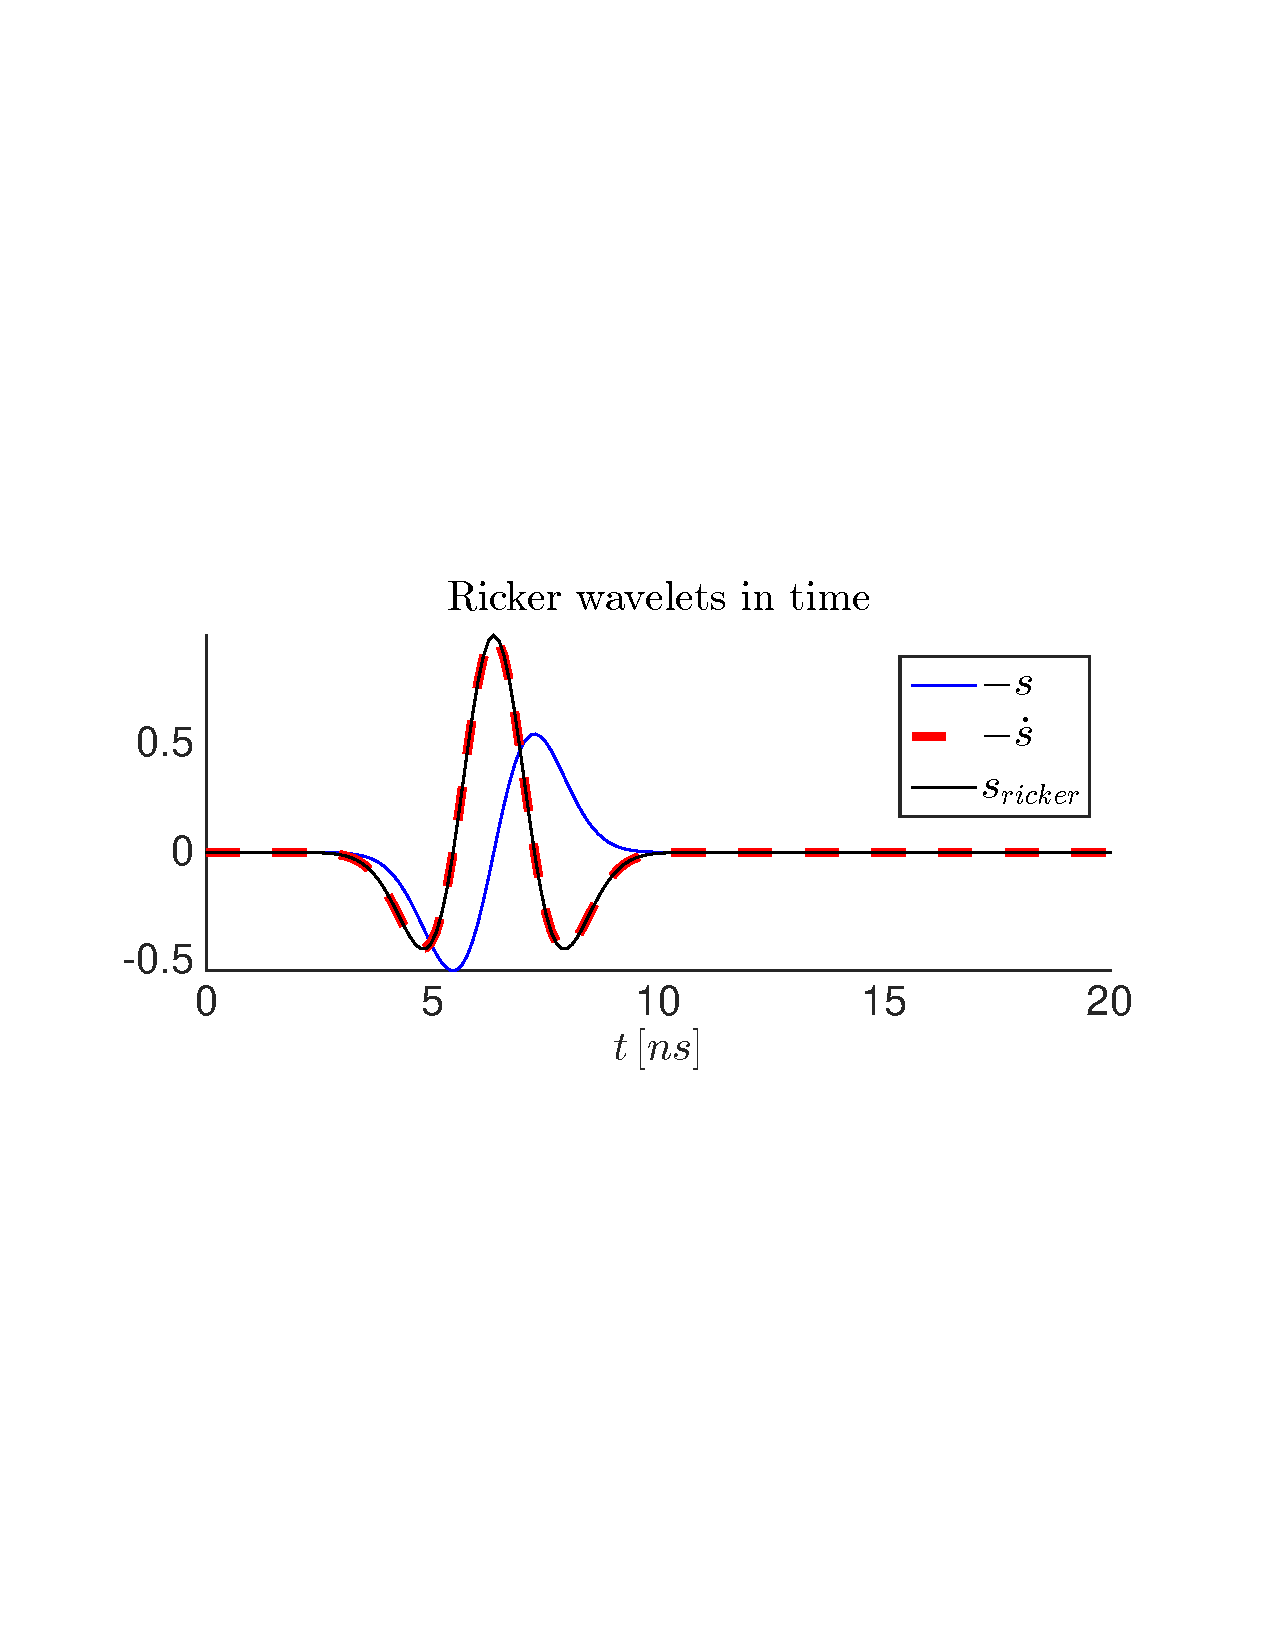
\includegraphics[trim={60 280 60 280},clip,width=0.6\textwidth]{pics/ricker-time-formula.pdf}\\~\\
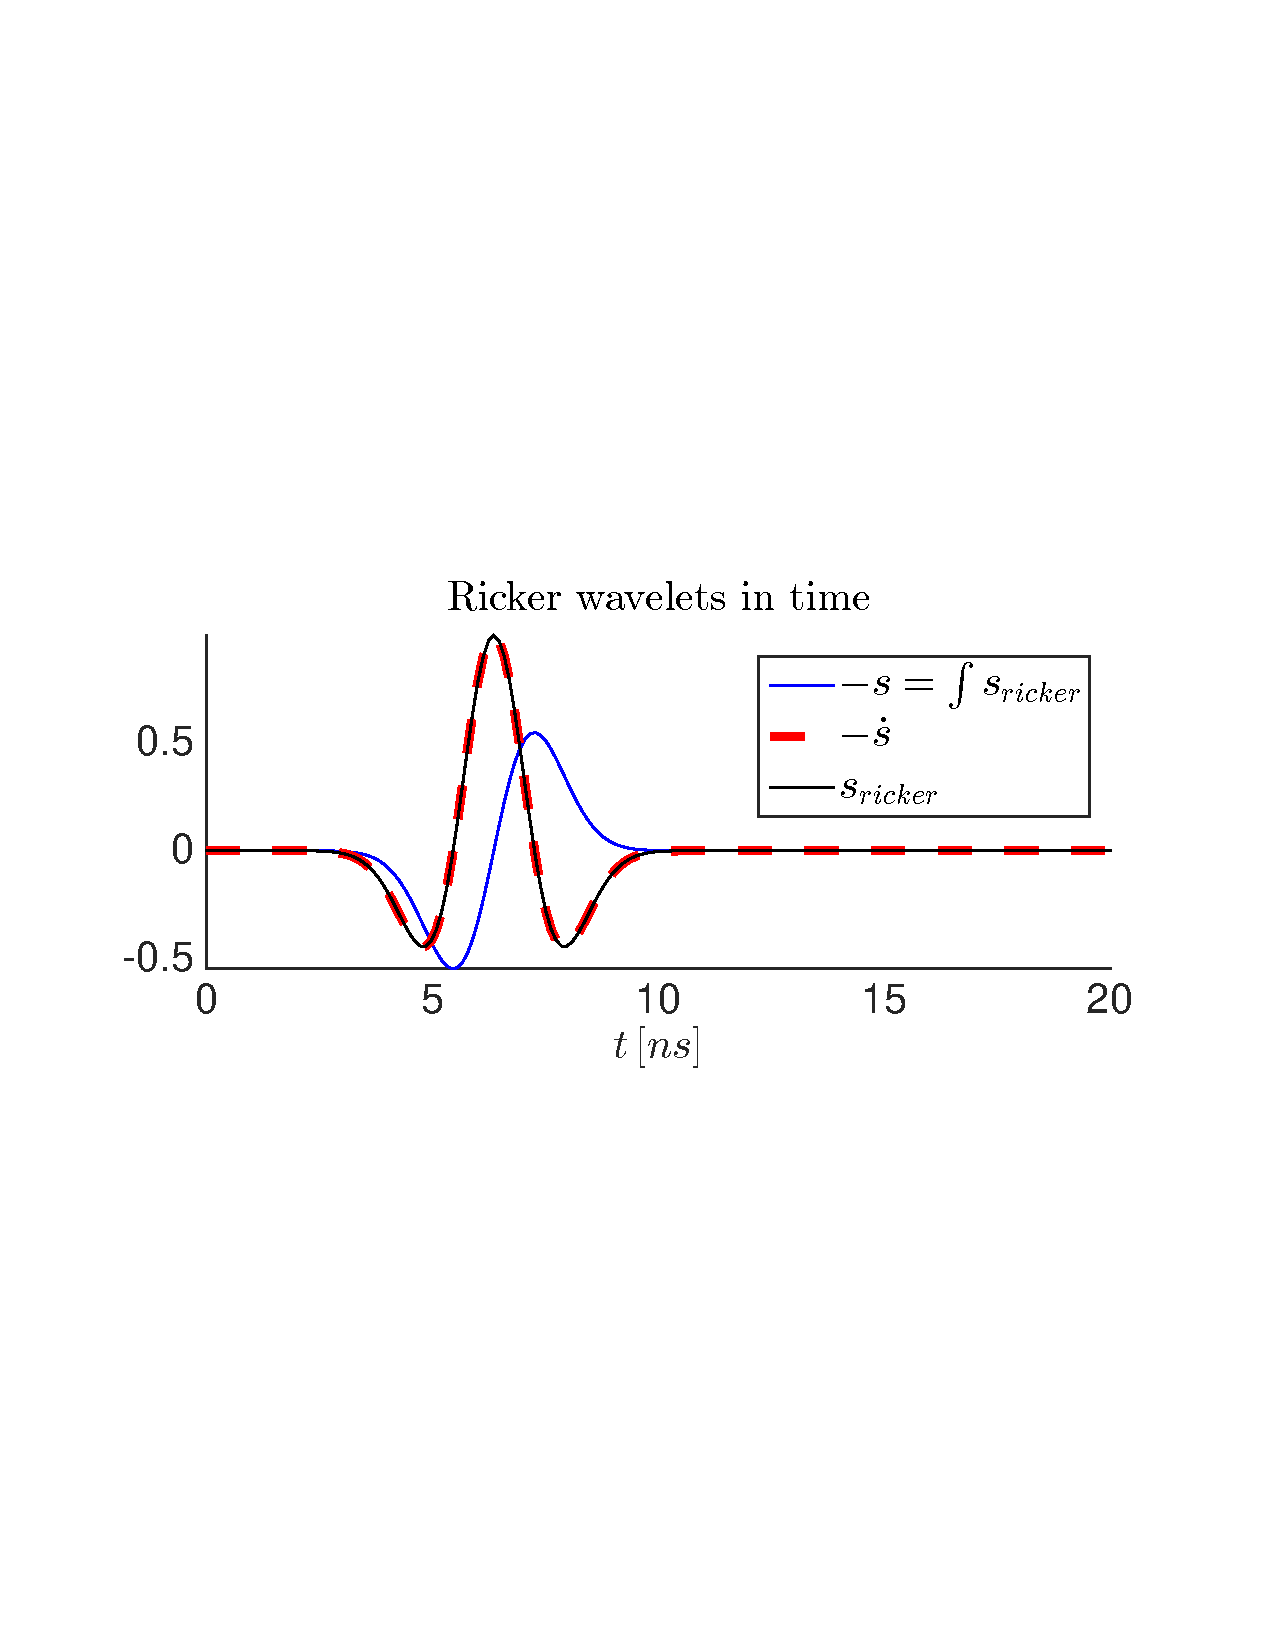
\includegraphics[trim={60 280 60 280},clip,width=0.6\textwidth]{pics/ricker-time-integral.pdf}\\~\\
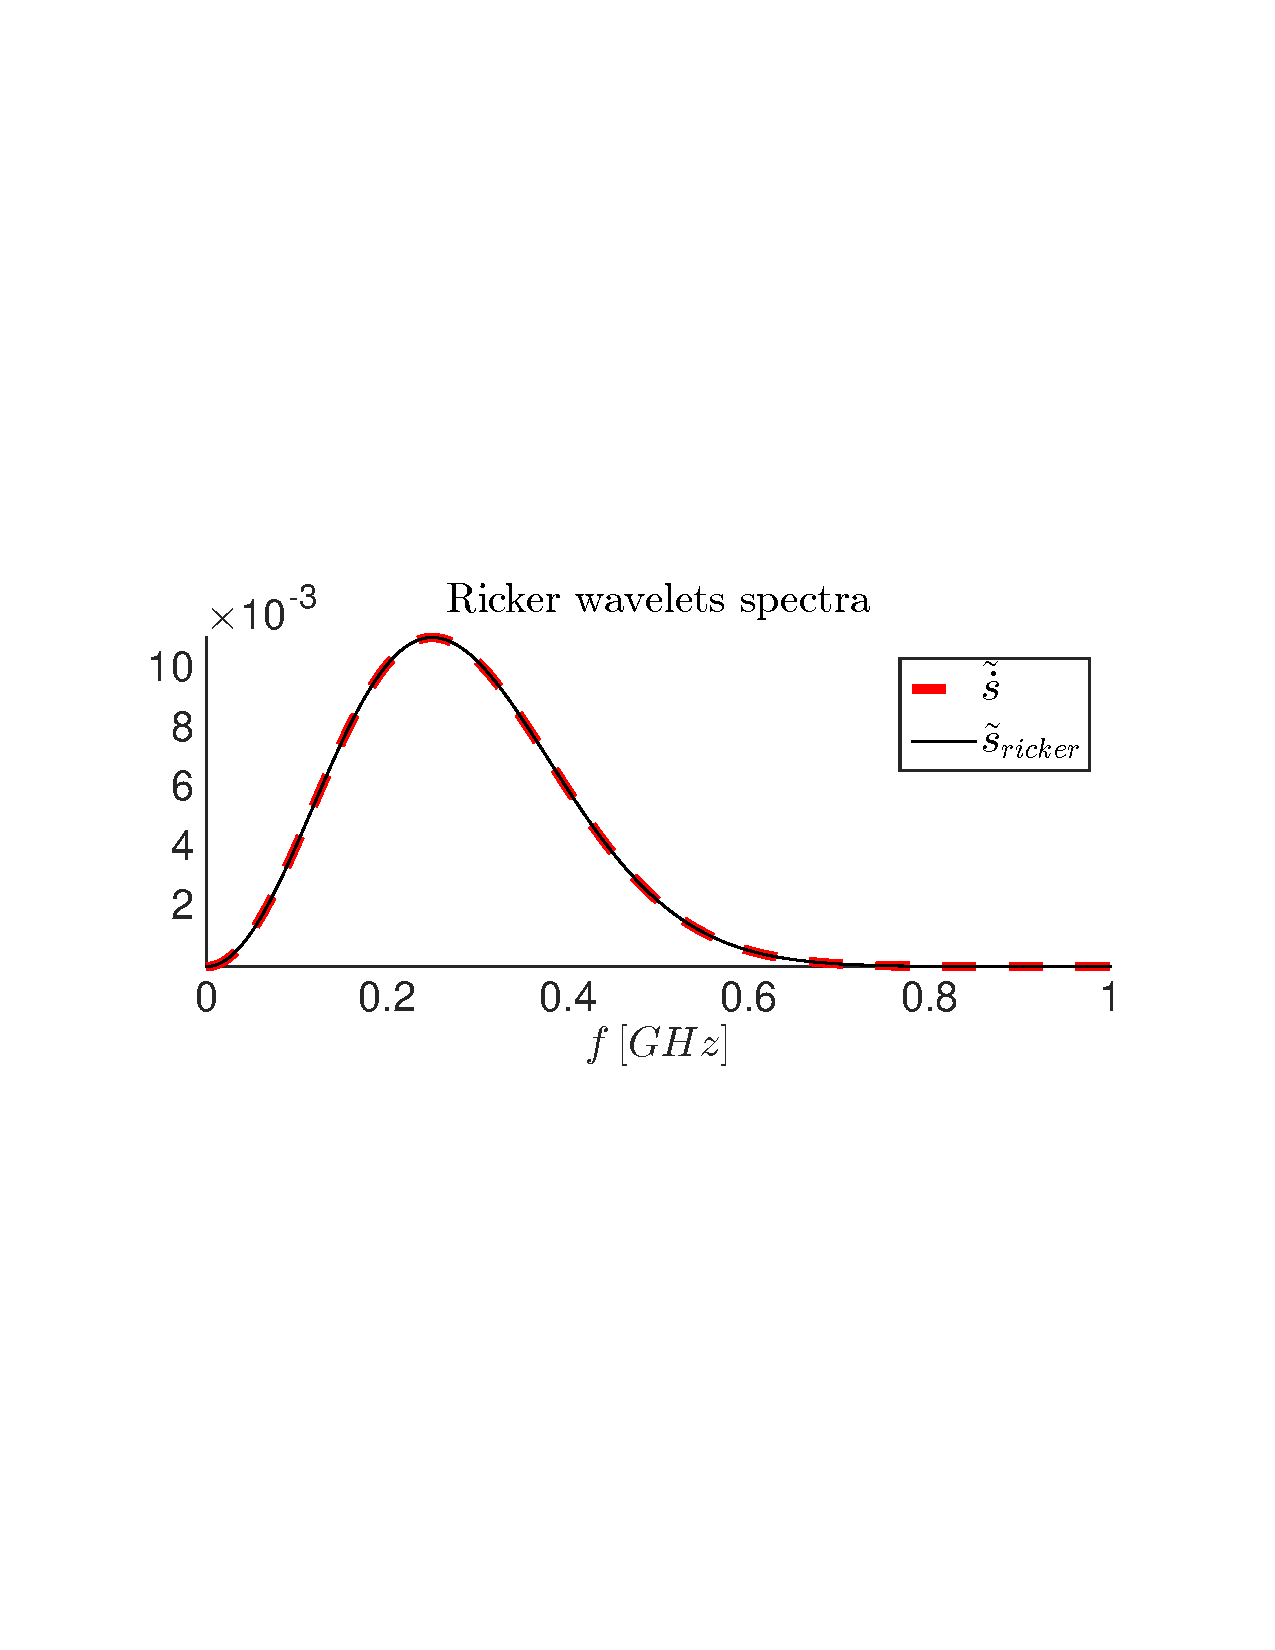
\includegraphics[trim={60 280 60 280},clip,width=0.6\textwidth]{pics/ricker-spectra.pdf}
\label{fig:ricker}
\caption{Analytical and numerical approximation of the Ricker wavelet in time and frequency.}
\end{figure}
%
%------------
% biblio
%------------
%\newpage
\bibliographystyle{plainnat}
\bibliography{w-2d-25d-src}
%\nocite{*}
\end{document}